\documentclass[]{article}

% Imported Packages
%------------------------------------------------------------------------------
\usepackage{amssymb}
\usepackage{amstext}
\usepackage{amsthm}
\usepackage{amsmath}
\usepackage{enumerate}
\usepackage{fancyhdr}
\usepackage[margin=1in]{geometry}
\usepackage{graphicx}
\usepackage{extarrows}
\usepackage{setspace}
\usepackage{placeins}
%------------------------------------------------------------------------------

% Header and Footer
%------------------------------------------------------------------------------
\pagestyle{plain}  
\renewcommand\headrulewidth{0.4pt}                                      
\renewcommand\footrulewidth{0.4pt}               
%------------------------------------------------------------------------------

% Title Details
%------------------------------------------------------------------------------
\title{Deliverable \#2 Template}
\author{SE 3A04: Software Design II -- Large System Design}
\date{}                               
%------------------------------------------------------------------------------

% Document
%------------------------------------------------------------------------------
\begin{document}

\maketitle	

\section{Introduction}
\label{sec:introduction}
% Begin Section

This section should provide an brief overview of the entire document.

\subsection{Purpose}
\label{sub:purpose}
% Begin SubSection
\begin{enumerate}[a)]
	\item Delineate the purpose of the document
	\item Specify the intended audience for the document
\end{enumerate}
% End SubSection

\subsection{System Description}
\label{sub:system_description}
% Begin SubSection
\begin{enumerate}[a)]
	\item Give a brief description of the system. This could be a paragraph or two to give some context to this document.
\end{enumerate}
% End SubSection

\subsection{Overview}
\label{sub:overview}
% Begin SubSection
\begin{enumerate}[a)]
	\item Describe what the rest of the document contains 
	\item Explain how the document is organised
\end{enumerate}
% End SubSection

% End Section

\section{Use Case Diagram}
\label{sec:use_case_diagram}
% Begin Section
\begin{figure}[!ht]
	\centering
	\includegraphics[scale=1]{UseCaseDiagram.png}
	\caption{Use Case Diagram}
\end{figure}
\begin{description}
	\item[View Previous Searches] The user must be able to review their previous searches. All searches should be saved so that they may be displayed in this list. The data saved should consist of the inputs entered to return the result.
	\item[Get More Song Info] Each song result is linked to more detailed information about the artist and song. The user should have access to this more detailed information on request. This use case cannot be executed unless a song is searched for first.
	\item[Search for Song] The user can search for a song based on the inputs given.
	\item[Input] This use case is a generic use case that is extended by more specific input fields. These fields include Tempo Input, Lyric Input and Artist Input.
	\item[Tempo Input] To input a tempo the user must tap on the screen at the desired tempo. This tempo is converted to a measurement in BPM for searching.
	\item[Lyric Input] To input lyrics users will have the option to type some lyrics into the search field or speak into the device's microphone and translate their voice to text via the speech-to-text functionality. These lyrics are a sequence of words that can be found in the desired song.
	\item[Artist Input] The artist input is the name of the artist that preforms the desired song. To input the artist the user may type the name into the search field or speak into the device's microphone and translate their voice to text via the speech-to-text functionality.
	\item[Consult Experts] Experts will be consulted to attempt to identify the desired song. They will work together to combine their opinions to decide on a song.
	\item[Add/Remove Expert] The administrator may wish to take an expert out of the system or introduce an new expert. In order to do so they must contact the developer who will directly preform the switch. 
\end{description}
\FloatBarrier % Stop the figure from leaving the section
% End Section

\section{Analysis Class Diagram}
\label{sec:analysis_class_diagram}
% Begin Section
\subsection{Noun Extraction}
\begin{description}
	\item[user] No (outside of system)
	\item[previous searches] Yes (boundary class) PreviousSearchPage
	\item[searches] refers to search process, leads to the creation of controller class SearchController
	\item[success] Yes (boundary class) SearchSuccessPage or SearchResults
	\item[error] Yes (boundary class) SearchErrorPage
	\item[song info] Yes (entity class) SongInformation
	\item[input] refers to input process, leads to the creation of controller class InputController
	\item[tempo input] Yes (boundary class)
	\item[lyric input] Yes (boundary class)
	\item[artist input] Yes (boundary class)
	\item[song database] Yes (boundary class), Wrapper
\end{description}

\begin{figure}[!ht]
	\centering
	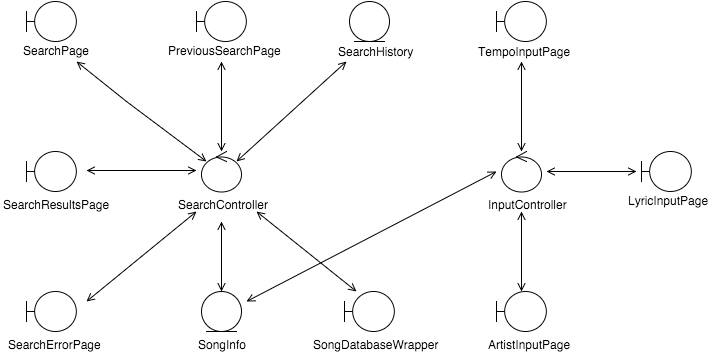
\includegraphics[scale=0.7]{Analysis_Class_Diagram.png}
	\caption{Analysis Case Diagram}
\end{figure}
\FloatBarrier
% End Section


\section{Architectural Design}
\label{sec:architectural_design}
% Begin Section

\subsection{System Architecture}
\label{sub:system_architecture}
% Begin SubSection
\begin{enumerate}[a)]
	\item A blackboard architectural design will be used.
	\item The system will primarily use the information obtained by 3 experts to determine a final result. The nature of this structure lends itself to the chosen type architecture.
\end{enumerate}
\begin{figure}[!ht]
	\centering
	\includegraphics[scale=1]{architecture.png}
	\caption{System Architecture Diagram}
\end{figure}
% End SubSection

\subsection{Subsystems}
\label{sub:subsystems}
% Begin SubSection
\begin{enumerate}[a)]
	\item \textbf{Artist Expert:} The expert charged with identifying songs associated with a given artist.
	\item \textbf{Lyric Expert:} The expert charged with identifying songs associated with a given lyric.
	\item \textbf{Tempo Expert:} The expert charged with identifying songs associated with a given tempo.
	\item \textbf{Blackboard:} The subsystem charged with combining data from all other subsystems and producing a final result for the user interface.
	\item \textbf{User Interface:} The subsystem charged with handling interactions with the user, including input and output.
\end{enumerate}
% End SubSection

% End Section
	
\section{Class Responsibility Collaboration (CRC) Cards}
\label{sec:class_responsibility_collaboration_crc_cards}
% Begin Section
This section should contain all of your CRC cards.

\begin{enumerate}[a)]
	\item Provide a CRC Card for each identified class
	\item Please use the format outlined in tutorial, i.e., 
	\begin{table}[ht]
		\centering
		\begin{tabular}{|p{5cm}|p{5cm}|}
		\hline 
		 \multicolumn{2}{|l|}{\textbf{Class Name:}} \\
		\hline
		\textbf{Responsibility:} & \textbf{Collaborators:} \\
		\hline
		\vspace{1in} & \\
		\hline
		\end{tabular}
	\end{table}
	
\end{enumerate}
% End Section

\appendix
\section{Division of Labour}
\label{sec:division_of_labour}
% Begin Section
Include a Division of Labour sheet which indicates the contributions of each team member. This sheet must be signed by all team members.
% End Section

\newpage
\section*{IMPORTANT NOTES}
\begin{itemize}
%	\item You do \underline{NOT} need to provide a text explanation of each diagram; the diagram should speak for itself
	\item Please document any non-standard notations that you may have used
	\begin{itemize}
		\item \emph{Rule of Thumb}: if you feel there is any doubt surrounding the meaning of your notations, document them
	\end{itemize}
	\item Some diagrams may be difficult to fit into one page
	\begin{itemize}
		\item It is OK if the text is small but please ensure that it is readable when printed
		\item If you need to break a diagram onto multiple pages, please adopt a system of doing so and thoroughly explain how it can be reconnected from one page to the next; if you are unsure about this, please ask about it
	\end{itemize}
	\item Please submit the latest version of Deliverable 1 with Deliverable 2
	\begin{itemize}
		\item It does not have to be a freshly printed version; the latest marked version is OK
	\end{itemize}
	\item If you do \underline{NOT} have a Division of Labour sheet, your deliverable will \underline{NOT} be marked
\end{itemize}


\end{document}
%------------------------------------------------------------------------------